% A workaround to allow relative paths in included subfiles
% that are to be compiled separately
% See https://tex.stackexchange.com/questions/153312/subfiles-inside-a-subfile-using-relative-paths
\providecommand{\main}{..}
\documentclass[\main/thesis.tex]{subfiles}

\begin{document}

\chapter{Method}
\label{cha:method}
\nelson{avoid passive voice}
This chapter discusses the contributed implementation of a high-performance and library-free matrix-matrix multiplication algorithm which makes use of \gls{mma}.
Due to its implementation in the LLVM compiler framework, the method has immediate performance-enhancing potential on the \gls{power10} platform.

\section{Intrinsics in LLVM}
An \gls{intrinsic} is a function available in an \gls{ir} and is therefore not directly available in higher-level languages.
Select \glspl{intrinsic} are available in higher-level languages in the form of a \gls{builtin}, though no \glspl{builtin} are used in this work.\footnotemark
\footnotetext{Some compilers use this terminology differently; these are the definitions according to \gls{llvm}.}
These functions' most important role is to symbolise the concept of a common operation in a representation that must lowered to many disparate forms while maintaining efficiency and correctness.
They are therefore not platform-specific but their lowering may be if the semantics necessitate it or if the maintainer wants to provide a more efficient version.
For example, the \gls{llvm} \gls{intrinsic} \code{llvm.vector.reduce.add.*} may be generically lowered to a series of vector operations at the \gls{ir} level, or, if the \gls{isa} provides a reduction instruction, it could be lowered more efficiently by the backend.

\subsection{Intrinsic Format}
Within \gls{llvm} \gls{ir}, \glspl{intrinsic} appear simply as external function declarations whose names are prefixed with ``\code{llvm.}''.
Names within \gls{llvm} are permitted to contain periods, a feature that \glspl{intrinsic} uses to \gls{mangle}  families of \glspl{intrinsic}.
Families arise from the need to provide generic \glspl{intrinsic} to a strongly typed language where overloading is not allowed.
For instance, consider the \code{llvm.smax.*} \gls{intrinsic} which takes two signed integers of the same type and returns the largest.
The \gls{llvm} documentation uses the ``\code{.*}'' suffix to represent the \glslink{mangle}{mangled} portion of the name.
An actual definition will replace the asterisk with a type name; if the function is generic in multiple places (return value, arguments) then the other type names will be appended and separated with more periods.
The \code{llvm.smax.*} \gls{intrinsic} only has one generic type.
\rlst{intrinsics} shows a declaration for a scalar 32-bit integer, typed and \glslink{mangle}{mangled} as \code{i32}, as well as for a length-four vector of 32-bit integers, typed as \code{<4 x i32>} and \glslink{mangle}{mangled} as \code{v4i32}.

\begin{lstlisting}[caption={[Example Inrinsic Declarations]A set of basic intrinsic declarations~\autocite{llvmLangref}.},
      label=lst:intrinsics,numbers=none,language=llvm,float,columns=flexible]
declare i32 @llvm.smax.i32(i32 %a, i32 %b)
declare <4 x i32> @llvm.smax.v4i32(<4 x i32> %a, <4 x i32> %b)
\end{lstlisting}

\section{The \texorpdfstring{\code{llvm.matrix.multiply.*}}{llvm.matrix.multiply.*} Intrinsic}
\label{sec:matMulInt}
\bk{Discuss the input vectors already being loaded.}
The \code{llvm.matrix.multiply.*} \gls{intrinsic} existed prior to this work and warrants a brief explanation to provide context~\autocite{llvmLangref}.
The \gls{intrinsic} has three generic types: the return-value type and the type of the two input matrices.
Each of the three matrices is typed as flattened vectors and therefore the signature requires three extra arguments to describe the dimensions as in \matmul{m}{d}{n}.

The original implementers required that input dimensions be statically known constants.
As well, those familiar with the analogous \gls{blas} routines may notice that arguments describing data-access order are conspicuously absent.
\nelson{Is column-major order referring to  the storage order or to the access order in this sentence?}
The original interface assumes that all matrices are column-major order.
Users may include a specific flag in their compiler invocation to change this setting to row-major order.
\nelson{"This"}
This means that a user may not mix data orientations within their program.
\rlst{matMulIntr} provides an example declaration and invocation of the intrinsic which computes \matmul{8}{5}{16}.

\begin{lstlisting}[caption={[Example Declaration and Use of \code{llvm.matrix.multiply.*}]An example declaration and usage of the \code{llvm.matrix.multiply.*} intrinsic.},
      label=lst:matMulIntr,language=llvm,float,columns=flexible]
declare <128 x float>
  @llvm.matrix.multiply.v128f32.v40f32.v80f32(
    <40 x float>, <80 x float>, i32, i32, i32
  )

define void @foo() {
  ; Declaration and construction of %A and %B...
  %C = call <128 x float>
    @llvm.matrix.multiply.v128f32.v40f32.v80f32(
      <40 x float> %A, <80 x float> %B, i32 8, i32 5, i32 16)
    )
  ; Function continues...
}
\end{lstlisting}

During lowering, the \code{call} statement is replaced with a series of \gls{llvm} \gls{ir} vector operations by the \code{LowerMatrixIntrinsics} pass.
This version of the lowering is what is referred to as the default ``vectorisation'' method.
Because the dimensions of the operation are known statically, the computation is completely unrolled: no loops will be generated.
Such a lowering is ideal because it removes the need for loop analysis and allows later passes to further vectorise or pipeline the operation.
This property makes it ideal for creating small and efficient kernels focused on efficient computation.
\bk{I'm not sure I need to expand on the vectorisation lowering. It's laid out very simply here, but more info may help contrast more.}

\nelson{kernels cannot be used with kernels....}
These kernels, because fully unrolling them creates a large amount of code, cannot be used with large kernels.
For example, unrolling a kernel for \matmul{128}{128}{128} takes several minutes of compilation time and results in an \gls{ir} file slightly larger than a gigabyte with over 12 million lines.
\nelson{"this"}
Producing a binary from this has never been accomplished due to the inordinate compilation time.
Therefore, wrapping the kernel in an outer kernel, which breaks down the operation while efficiently handling memory movement, is a necessity.
For further discussion see \bk{PACT paper or section N}.

\section{An Alternate Lowering Using MMA}
\label{sec:alternateLowering}
We look to implement an improvement to this lowering on the \gls{power} platform using \gls{mma}.
Content in \rsec{baseCase}, \rsec{dataTypes}, and \rsec{arbitraryDims} is derived from work currently under revision~\autocite{kuzma2021fast}.

\bk{
  I'm not sure this is enough context for the upcoming section; it's not apparent why the output is $8 \times 16$.
  I am, however, writing this before having finished the explanation of MMA which should be in a previous chapter.
}
\nelson{Preceding what?}
This preceding work focused on a lowering for floating point values when computing \matmul{8}{5}{16}.
The $8 \times 16$ output size is exactly the output dimensions produced when fully utilising the architecture's available accumulators.
This property made it the ideal size for the intrinsic's role as a tight inner kernel.
Nevertheless, these restrictions create a simple scenario enabling a foundational understanding of this thesis' core algorithm; removing these restrictions is discussed in \rsec{dataTypes}, \rsec{arbitraryDims}, and \rsec{arbitraryOrder}.

\subsection{Base Case}
\label{sec:baseCase}
\todo{Find a better title.}
In addition to the software constraints described in \rsec{matMulInt}, an efficient MMA lowering must take into account the following hardware constraints:
\begin{enumerate*}[itemjoin*={{ and }}, label=\fbox{\arabic*}]
  \item eight accumulators are available per thread and for each accumulator that is used, the usage of four \glspl{vsr} are blocked;
  \item there are 64 \glspl{vsr}, thus if eight accumulators are used, there are 32 \glspl{vsr} remaining to contain data from input matrices;
  \item two multiply-and-accumulate outer-product instructions can be issued per single cycle;
  \item the issue-to-issue latency for the same accumulator is four cycles;
  \item spilling an accumulator to memory is an expensive operation because it requires an instruction to disassemble the accumulator into four \glspl{vsr}, four vector store instructions and, later, four vector load instructions.
\end{enumerate*}

\begin{figure}[t]
  \centering
  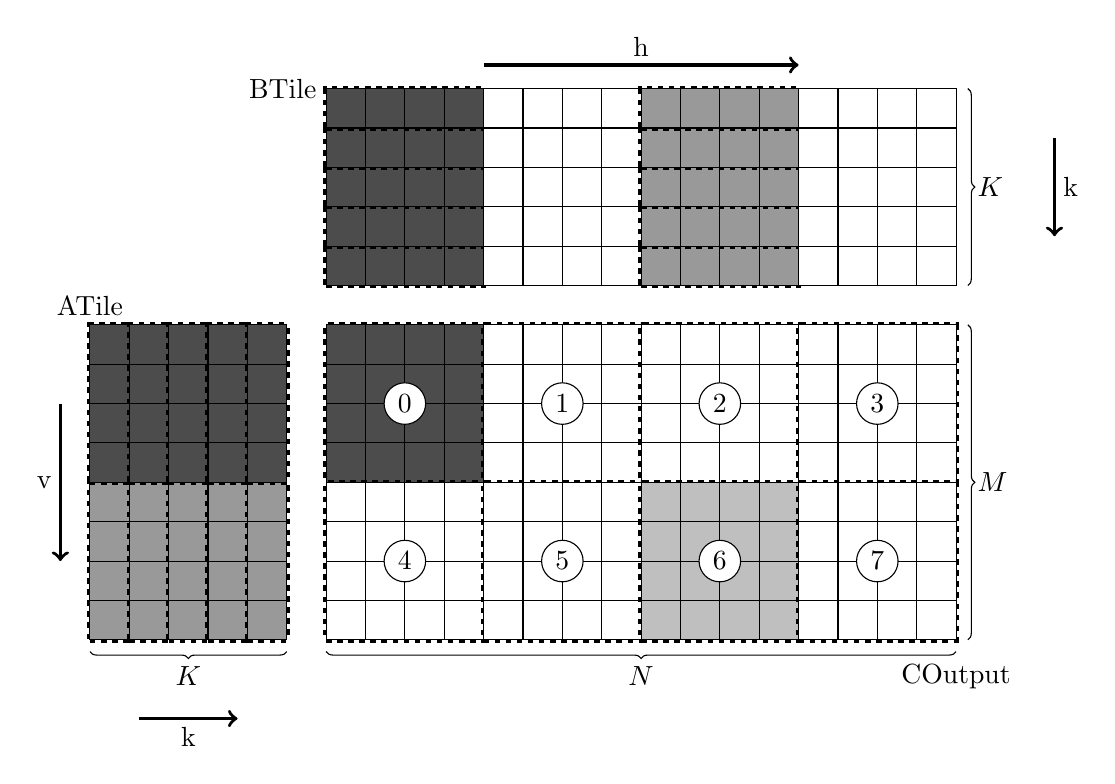
\begin{tikzpicture}[scale=1/2]
    % Grids.
    \foreach \x/\y/\dx/\dy/\c/\o in
        { 0/0/1/4/black!40!white/1,1/0/1/4/black!40!white/1,2/0/1/4/black!40!white/1, % A1,1-3
          3/0/1/4/black!40!white/1,4/0/1/4/black!40!white/1, % A1,4-5
          0/4/1/4/black!70!white/1,1/4/1/4/black!70!white/1,2/4/1/4/black!70!white/1, % A2,1-3
          3/4/1/4/black!70!white/1,4/4/1/4/black!70!white/1, % A2,2-5
          6/9/4/1/black!70!white/1,6/10/4/1/black!70!white/1,6/11/4/1/black!70!white/1, % B1,1-3
          6/12/4/1/black!70!white/1,6/13/4/1/black!70!white/1, % B1,4-5
          10/9/4/1/white/0,10/10/4/1/white/0,10/11/4/1/white/0, % B2,1-3
          10/12/4/1/white/0,10/13/4/1/white/0, % B2,4-5
          14/9/4/1/black!40!white/1,14/10/4/1/black!40!white/1,14/11/4/1/black!40!white/1, % B3,1-3
          14/12/4/1/black!40!white/1,14/13/4/1/black!40!white/1, % B3,4-5
          18/9/4/1/white/0,18/10/4/1/white/0,18/11/4/1/white/0, % B4,1-3
          18/12/4/1/white/0,18/13/4/1/white/0, % B4,4-5
          6/4/4/4/black!70!white/1,10/4/4/4/white/1,14/4/4/4/white/1,18/4/4/4/white/1, % C1,2,3,4
          6/0/4/4/white/1,10/0/4/4/white/1,14/0/4/4/black!25!white/1,18/0/4/4/white/1} % C5,6,7,8
    {
      \draw[step=1, shift={(\x, \y)}] (0, 0) grid +(\dx, \dy);
      \ifnum\o=1
        \draw[line width=2,dotted,shift={(\x, \y)}] (0, 0) -- (\dx, 0) -- (\dx, \dy) -- (0, \dy) -- cycle;
      \fi
      \pgfmathsetmacro{\yMax}{\dy-1}
      \pgfmathsetmacro{\xMax}{\dx-1}
      \foreach \yIdx in {0,...,\yMax} {
        \foreach \xIdx in {0,...,\xMax} {
          \pgfmathsetmacro{\xc}{\x+\xIdx}
          \pgfmathsetmacro{\yc}{\y+\yIdx}
          \draw[fill=\c] (\xc, \yc) -- +(1, 0) -- +(1, 1) -- +(0, 1) -- cycle;
        }
      }
    }

    % Arrows.
    \draw[->,line width=1.25] (-0.75, 6) -- node[left=-.75] {\code{v}} +(0, -4);
    \draw[->,line width=1.25] (10, 14.6) -- node[above=-.75] {\code{h}} +(8, 0);
    \draw[->,line width=1.25] (1.25, -2) -- node[below=-.75] {\code{k}} +(2.5, 0);
    \draw[->,line width=1.25] (24.5, 12.75) -- node[right=-.75] {\code{k}} +(0, -2.5);

    % Matrix labels.
    \node[above] at (0, 8) {\code{ATile}};
    \node[left] at (6, 14) {\code{BTile}};
    \node[below=2] at (22, -0.25) {\code{COutput}};

    % Axis labels.
    \draw[decorate, decoration={brace, mirror}] (0, -0.3) -- node[below=2] {$K$} +(5, 0);
    \draw[decorate, decoration={brace, mirror}] (6, -0.3) -- node[below=2] {$N$} +(16, 0);
    \draw[decorate, decoration={brace, mirror}] (22.3, 0) -- node[right] {$M$} +(0, 8);
    \draw[decorate, decoration={brace, mirror}] (22.3, 9) -- node[right] {$K$} +(0, 5);

    % Tile labels.
    % \foreach \y in {0, 4} {
    %   \draw[decorate, decoration={brace}] (-0.15, \y) -- node[left=0.5, anchor=south, rotate=90] {\footnotesize strip} +(0, 4);
    % }
    % \foreach \x in {6, 10, 14, 18} {
    %   \draw[decorate, decoration={brace}] (\x, 14.15) -- node[above=0.5] {\footnotesize strip} +(4, 0);
    % }

    % Tile numbering.
    \foreach \x in {0, ..., 3} {
      \foreach \y in {0, 1} {
        \pgfmathsetmacro{\nx}{(\x + 2) * 4}
        \pgfmathsetmacro{\ny}{(1 - \y) * 4 + 2}
        \pgfmathsetmacro{\i}{int(\x + \y * 4)}
        \node[circle,draw=black,fill=white,inner sep=0, minimum size=15] at (\nx, \ny) {\i};
      }
    }
  \end{tikzpicture}
  \caption[Operand and Accumulator Layout in MMA]{Division of \code{ATile} and \code{BTile} into operands and \code{COutput} into MMA accumulators.}
  \label{fig:intrinsic}
\end{figure}

\bk{Consider highlighting an argument register in different way now that the diagram is larger.}
\rfig{intrinsic} illustrates how \code{COutput} is divided into portions that are assigned to the MMA accumulators.
\code{ATile}, \code{BTile}, and \code{COutput} are represented in two dimensions to illustrate the position of the elements in the matrices.
Each small square in the figure represents one 32-bit element of a matrix.
A circled number indicates that the corresponding portion of \code{COutput} is assigned to that accumulator number.
When the intrinsic is executed each accumulator computes $K$ outer products using a multiply-and-add operation.
The two tones of gray colour in \rfig{intrinsic} illustrate that a strip of \code{ATile} and a strip of \code{BTile} are used for the accumulation of each portion of \code{COutput}.
Each strip is reused for all the accumulations in the same row or column of accumulators.
Each outer-product computation needs two four-element operands, one from \code{ATile} and one from \code{BTile}.
These operands are surrounded by dashed lines for the two accumulations highlighted in gray.
The arrows indicate how the loop indices in \ralg{intrinsic} iterate for the example in the figure.

\ralg{intrinsic} describes the lowering of the intrinsic computation for MMA.
This is the algorithm within the compiler that produces \gls{llvm} \gls{ir}, not the code executed on the target machine.
The produced code and its complications are discussed in \rsec{unrolled}.

The compile-time constants \code{V} and \code{H} (used on lines~\ref{VextractLoop}, \ref{HextractLoop}, \ref{computeLoop1}, \ref{computeLoop2}) specify the layout of the accumulators for the computation.
Given constraint \fbox{1}, the largest amount of data reuse can be obtained when \code{V = 2} and \code{H = 4} or vice versa (see \rfig{intrinsic}).
The only other configuration with full accumulator usage (\code{V = 1}, \code{H = 8}) uses more operand registers for a single accumulation -- nine instead of six -- and demonstrates reuse along only a single axis.
These constants in the compiler generalise the lowering and make it applicable to future architectures where the ideal arrangement to increase data reuse may be different from the $2 \times 4$ arrangement in the \gls{power10} processor.

\begin{algorithm}[t]
  \caption[Algorithm for lowering \code{llvm.matrix.multiply}]{Algorithm for lowering \code{llvm.matrix.multiply} with \gls{mma}.}
  \label{alg:intrinsic}
  \begin{algorithmic}[1]
    \Function{\code{llvm.matrix.multiply}}{ATile, BTile, $N$, $K$, $M$}
    \State MMAIntrinsic~$\gets$~intrinsic chosen based on element type\label{chooseIntrinsic}
    \State COutput~$\gets$~$N \times M$ empty array\label{createC}
    \State Accs~$\gets$~$V \times H$ ACCs assembled and initialised to zero\label{zeroAccs}
    \For{$\text{\code{k}}=0$ \textbf{to} $K-1$}\label{unrollLoopStart}
      \State AOps~$\gets$~$V$ empty vector operands
      \State BOps~$\gets$~$H$ empty vector operands
      \For{$\text{\code{v}}=0$ to $V-1$}\label{VextractLoop}
        \State AOps[\code{v}]~$\gets$~Extract operand at ATile[$\text{\code{v}} \times 4$][\code{k}]\label{aOps}
        \EndFor
      \For{$\text{\code{h}}=0$ to $H-1$}\label{HextractLoop}
         \State BOps[\code{h}]~$\gets$~Extract operand at BTile[$\text{\code{h}} \times 4$][\code{k}]\label{bOps}
      \EndFor
      \For{$\text{\code{v}}=0$ to $V-1$}\label{computeLoop1}
        \For{$\text{\code{h}}=0$ to $H-1$}\label{computeLoop2}
          \State createCall(MMAIntrinsic, {Accs[\code{v}][\code{h}], AOps[\code{v}], BOps[\code{h}]})\label{intrinsicCallCreate}
        \EndFor
      \EndFor
    \EndFor\label{accLoopEnd}
    \State Disassemble ACCs and store VSRs into COutput\label{disStore}
    \State \Return COutput\label{return}
    \EndFunction
  \end{algorithmic}
\end{algorithm}

First, on line~\ref{chooseIntrinsic}, an \gls{mma} intrinsic is chosen based on the element type of the operation\footnotemark (\eg \code{float}, \code{i32}).
\footnotetext{
  This is an operation internal to the matrix multiplication meaning all negations have been applied prior to the intrinsic.
  Therefore, the positive multiply, positive accumulate variant is always chosen.
}
Next, an array is created to contain the eventual output (line~\ref{createC}) followed by assembling zeroed-out accumulators (line~\ref{zeroAccs}).
The following loop (line~\ref{unrollLoopStart}) iterates from $0$ to $K-1$, extracting operands and performing accumulations.
For each value of \code{k}, using the accumulator assignment shown in \rfig{intrinsic}, the algorithm extracts two operands from \code{ATile} (lines~\ref{VextractLoop}-\ref{aOps}) and four operands from \code{BTile} (lines~\ref{HextractLoop}-\ref{bOps}).
For $\text{\code{k}}=0$ the operands are extracted from the leftmost column of \code{ATile} and from the topmost row of \code{BTile} in \rfig{intrinsic}.
The algorithmic presentation in \ralg{intrinsic} uses the notation \code{ATile[}$\text{\code{v}} \times 4$\code{][k]} and \code{BTile[}$\text{\code{h}} \times 4$\code{][k]} to denote the index where operand vector starts.
These operands are extracted to virtual IR registers; the actual \glspl{vsr} to be used will be determined later by a register-allocation pass.

In \rfig{intrinsic} each operand is formed by four elements and, once extracted, occupies one 128-bit \gls{vsr}.
Given constraints \fbox{1} and \fbox{2}, with the choice of $K = 5$, there are enough non-blocked \glspl{vsr} to contain all the thirty operands needed for the computation illustrated in \rfig{intrinsic}.
Thus, laying out the accumulators in this $2 \times 4$ pattern maximises the reuse of values loaded into the \glspl{vsr}: operands extracted from \code{ATile} are reused four times and operands extracted from \code{BTile} are reused two times.

Once this iteration's operands are extracted, the algorithm then iterates over the accumulators (lines~\ref{computeLoop1}-\ref{computeLoop2}) and creates a call to the \gls{mma} \gls{intrinsic}, computing a single accumulation in each.
Following constraint \fbox{3}, two outer-product instructions can be issued each cycle.
Four pairs of accumulators can be scheduled before circling back to the first pair, thus satisfying constraint \fbox{4}.
The assignment of a portion of \code{COutput} to a single accumulator eliminates the need to spill accumulators, thus increasing the performance according to constraint \fbox{5}.

\subsection{The Resulting IR}
\label{sec:unrolled}
\bk{Find a better section name.}
As discussed in \rsec{matMulInt}, the fully unrolled \gls{ir} code for the \gls{lowering} of an \gls{intrinsic} can be extremely long.
\rlst{unrolled} presents the code resulting from unrolling \matmul{8}{1}{16}.
The result has been simplified but preserves the process presented in \ralg{intrinsic}.
The listing shows all operations starting from the initialisation of the accumulators to the disassembling.
The matter of storing vectors to memory is easily addressed and so is left out for brevity.

\begin{lstlisting}[caption={[Example Lowering of \code{llvm.matrix.multiply.*}.]An example lowering of the \code{llvm.matrix.multiply.*} intrinsic for a $8 \times 1 \times 16$ computation.},
      label=lst:unrolled,language=llvm,basicstyle=\small\ttfamily,float,escapechar=|,columns=flexible,breaklines=true,breakatwhitespace=true]
  %ACC = call <512 x i1> @llvm.ppc.mma.xxsetaccz()|\label{accz}|
  %ATile.0_0 = shufflevector <8 x float> %ATile, <8 x float> undef, <4 x i32> <i32 0, i32 1, i32 2, i32 3>|\label{aShuffle1}|
  %ATile.0_4 = shufflevector <8 x float> %ATile, <8 x float> undef, <4 x i32> <i32 4, i32 5, i32 6, i32 7>|\label{aShuffle2}|
  %BTile.0_0 = shufflevector <16 x float> %BTile, <16 x float> undef, <4 x i32> <i32 0, i32 1, i32 2, i32 3>|\label{bShuffle1}|
  %BTile.0_4 = shufflevector <16 x float> %BTile, <16 x float> undef, <4 x i32> <i32 4, i32 5, i32 6, i32 7>
  %BTile.0_8 = shufflevector <16 x float> %BTile, <16 x float> undef, <4 x i32> <i32 8, i32 9, i32 10, i32 11>
  %BTile.0_12 = shufflevector <16 x float> %BTile, <16 x float> undef, <4 x i32> <i32 12, i32 13, i32 14, i32 15>|\label{bShuffle2}|
  %ACCProd.0_0.0 = call <512 x i1> @llvm.ppc.mma.xvf32gerpp(<512 x i1> %ACC, <4 x float> %ATile.0_0, <4 x float> %BTile.0_0)|\label{accsBegin}|
  %ACCProd.0_1.0 = call <512 x i1> @llvm.ppc.mma.xvf32gerpp(<512 x i1> %ACC, <4 x float> %ATile.0_0, <4 x float> %BTile.0_4)
  ...
  %ACCProd.1_3.0 = call <512 x i1> @llvm.ppc.mma.xvf32gerpp(<512 x i1> %ACC, <4 x float> %ATile.0_4, <4 x float> %BTile.0_12)|\label{accsEnd}|
  %ACCDis.0_0 = call { <4 x float>, <4 x float>, <4 x float>, <4 x float> } @llvm.ppc.mma.disassemble.acc(<512 x i1> %ACCProd.0_0.0)|\label{dissStart}|
  %ACCDis.0_1 = call { <4 x float>, <4 x float>, <4 x float>, <4 x float> } @llvm.ppc.mma.disassemble.acc(<512 x i1> %ACCProd.0_1.0)
  ...
  %ACCDis.1_3 = call { <4 x float>, <4 x float>, <4 x float>, <4 x float> } @llvm.ppc.mma.disassemble.acc(<512 x i1> %ACCProd.1_3.0)|\label{dissEnd}|
\end{lstlisting}

First, on line~\ref{accz} of \rlst{unrolled}, a call to the \gls{ppc} \gls{intrinsic} \code{xxsetaccz}\footnotemark.
\footnotetext{
  The latest version of the algorithm begins from a non-accumulating outer-product instruction (\rsec{matMulMMA}) instead of a \code{xxmtacc} or \code{xxsetaccz} (\rsec{assDis}).
  The \code{xxsetaccz} remains in this listing to connect with \ralg{intrinsic}.
}
Only a single assembly is required in the \gls{ir} because the \gls{ir} is in \gls{ssa} form.
Because the intrinsic takes no arguments and is functionally pure\footnotemark within the \gls{ir}, the result of multiple repeated calls are seen by the optimiser as identical and will be removed by a \gls{cse} pass.
\footnotetext{
A pure function is one which:
  \begin{enumerate*}[itemjoin*={{ and }}, label=\textbf{(\arabic*)}, after={.}]
    \item has no side effects (e.g. writes to memory)
    \item returns the same output given the same input
  \end{enumerate*}
}
Therefore, it is up to the register allocation pass to later recognise the need for and to provide multiple simultaneous accumulators.
Thus, all operations begin from the ``same'' zeroed out accumulator, at least within the \gls{ir}.

The \code{<512 x i1>} return type of \code{xxsetaccz} normally refers to a 512-length vector of one-bit integers.
However, backend developers have co-opted the type to represent an \gls{mma} accumulator when certain flags are set.
There also exists a separate type which represents a \gls{vsr} for use with \gls{mma} \glspl{intrinsic} but its use was removed from \rlst{unrolled} to facilitate reading\footnotemark.
\footnotetext{
  \glspl{vsr} are represented by \code{<16 x i8>}, a 16-element vector of bytes.
  In the true result \gls{ir}, shuffles produce four-element vectors of floats which are bit-casted (same bit-width) to the \gls{vsr} type which is then consumed by the intrinsics.
}

Line~\ref{aShuffle1} shows the extraction of the first operand from \code{ATile} via a shuffle instruction.
Conceptually, the shuffle instruction takes two equally sized vector operands, logically concatenates them, and labels each element from $0$ to $2N$.
A third argument, the shuffle mask, is a vector of labels defining which element from the concatenation should be in the output vector's same position.
For example, with two four-length vectors as arguments and a mask of \code{<i32 7, i32 3, i32 0>}, a shuffle would produce a three-element vector starting with the second vector's final element followed by the first vector's final and first elements.
Furthermore, the special value \code{undef} can be used to replace one of the input vectors to allow easily manipulation of the elements of a single vector.
Selecting an element from the \code{undef} vector results in undefined behaviour.

With this we can see that line~\ref{aShuffle1} combines \code{ATile} and \code{undef} and extracts the first four elements of \code{ATile}; the result variable is named \code{ATile.0_0} indicating the vector starts at $(0, 0)$.
The next four elements are extracted on line~\ref{aShuffle2} for the second operand vector.
All four operand vectors are extracted from \code{BTile} in a similar process on lines~\ref{bShuffle1}-\ref{bShuffle2}.

Outer products and accumulations begin on line~\ref{accsBegin} and end on line~\ref{accsEnd}.
Each operation takes an accumulator as the first argument and multiplies the two extracted operands found in the second and third arguments.
The \code{xvf32gerpp} intrinsic returns a value with type \code{<512 x i1>}, the accumulator type.
This represents the inputted accumulator with the operation accumulated on top.
In this first iteration, the zeroed out accumulator will be duplicated for each operation.
In the next iteration of accumulations, the returned accumulators will be used as the first argument.
This process continues with each accumulation, creating a chain of return values to arguments, effectively showing the accumulation process.

\subsubsection{Complications}
\label{sec:complications}
\bk{Discuss code gen issues from assembly.}
\bk{Discuss $K=5$ being incorrect.}
\bk{Discuss ``correct'' operand access order.}

\subsection{Other Data Types}
\label{sec:dataTypes}
\bk{Do I need to cut some of this out now that it's explained in \rsec{matMulMMA}?}
The presentation so far has assumed 32-bit data types where each operand \gls{vsr} contains 4 elements and an MMA instruction computes a rank 1 update, computing and accumulating a single outer product.
Halving the data-type size doubles the number of elements in each \gls{vsr} and doubles the rank of the update.
For example, for a 16-bit data type, MMA computes a rank 2 update while an 8-bit data type computes a rank 4 update.
The packing of more elements into a single \gls{vsr} and the accumulation of multiple outer products by a single MMA instruction requires changes \ralg{intrinsic}.
Let $p$ be the number of outer products performed by an MMA instruction --- \ie the rank of the update.
Now the step size of the loop on line~\ref{unrollLoopStart} must be $p$ because, in \rfig{intrinsic}, $p$ rows of a vertical section of \code{BTile} and $p$ columns of horizontal section of \code{ATile} are packed into each \gls{vsr}.
The extraction of operands in lines~\ref{aOps} and \ref{bOps} is now a strided access.
For instance, for $p=2$ (16-bit data types), four consecutive elements are extracted from row $k$ and four consecutive elements are extracted from row $k+1$ to form the 128-bit \gls{vsr}.
The length of $K$ must increase by $p$ times to provide enough data to populate the \glspl{vsr}.
The effect is that more partial-product accumulations can be computed per micro-kernel invocation given the same number of assemblies and disassemblies because the number of multiplications per outer product increases by $p$.

For the double-precision floating-point data type, an accumulator contains $4 \times 2$ 64-bit elements.
The operand extracted from \code{ATile} is placed into a combination of two \glspl{vsr} that each contain two elements, collectively four, while the operand extracted from \code{BTile}, now only two elements, is placed into a single 128-bit \gls{vsr}.
Therefore, for double-precision floats, the value of $N$ should be reduced by half to reflect the number of \glspl{vsr} available.
With this reduction, an \code{ATile} tile occupies 16 \glspl{vsr} and a \code{BTile} tile also occupies 16 \glspl{vsr}.
The extraction of operands into vector registers in lines~\ref{aOps} and~\ref{bOps} of \ralg{intrinsic} must be changed accordingly.

\subsection{Arbitrary Values for \texorpdfstring{$M$}{M}, \texorpdfstring{$K$}{K}, \texorpdfstring{$N$}{N}}
\label{sec:arbitraryDims}
\bk{Coutput created before K makes a lot more sense with the arbitrary dimensions}
% For simplicity, the presentation of the algorithms assumed that $N$ and $K$ are selected so that a tile of matrix \code{A} and a tile of matrix \code{B} have the exact dimensions needed for the accumulator arrangement shown in \rfig{intrinsic}.
Until now, the algorithms have used values of $M$ and $N$ selected such that a micro kernel with the accumulator arrangement shown in \rfig{intrinsic} could be computed with a single set of assemble and disassemble instructions.
However, the implementation of \ralg{intrinsic} in LLVM must handle any \code{llvm.matrix.multiply} intrinsic created by any compilation path and thus must handle arbitrary values for $M$, $N$ and $K$.

To handle larger values of $M$ and $N$, the micro-level code-lowering algorithm has an additional outer double-nested loop that logically divides the \code{CVec} tile into $8 \times 16$-element sections as shown in \rfig{intrinsic}.
Each of these sections can then be handled as shown in \ralg{intrinsic}.
The disadvantage of an input size that spans multiple accumulator sections is that the extraction of data into vector registers becomes more complex.
For example, consider a 32-bit data multiplication as shown \rfig{intrinsic} but with the values of $N$ and $M$ double of what is shown in the figure.
The rows of \code{ATile} and \code{BTile} shown in \rfig{intrinsic} are now a portion of the rows of larger tiles and the data extraction must gather the correct data into the vector registers that will be used by the accumulators.
This data gathering adds additional code and may impact access locality if the tiles are large enough.

\subsection{Arbitrary Access Order}
\label{sec:arbitraryOrder}
The code-lowering algorithm also supports inputs and outputs in any access order through modifications to the functions that extract operands and store the results in the accumulators to memory.

Operands in \gls{vsr} from \code{ATile} must always be in row-major order while operands from \code{BTile} must always be in column-major order.
Without loss of generality, consider extracting an operand from \code{Atile}.
Using the notation from \rsec{dataTypes}, the final operand \gls{vsr} must be a row-major $4 \times p$ matrix.
Given a column-major matrix argument to the intrinsic, we can extract $p$ length-four vectors from the columns and then interleave (also called zip) them to produce the \gls{vsr}.
The interleaving essentially converts the data access order from column major to row major.
If the operand matrix is row major, we can extract four length-$p$ vectors from the rows and then concatenate to produce the \gls{vsr}.
In the case of 32- or 64-bit data types, these operations appear to the contrary, but the truth remains that an argument \gls{vsr} extracted from \code{ATile} is actually four one-element rows not one four-element column.

\bk{
  I have a feeling that I'll need a diagram proving that transposition == access order change in regards to underlying element order.
  Having this means I'll probably rewrite this entire paragraph, it feels pretty clumsy as is.
}
Accumulators can change orientations using a simple mathematical theorem: given matrices $A, B, C$, if $C = AB$ then $C^T=B^TA^T$.
This fact coupled with the knowledge that transposition and access order change is the same operation regarding element movement in memory, we begin by adding data ordering information to the equations: if $C_{RM}=A_{RM}B_{CM}$ then $C^T_{RM}=B^T_{CM}A^T_{RM}$.
Now, focusing on the second equation, we can reduce the transpositions to changes in the data ordering to produce $C_{CM}=B_{RM}A_{CM}$.
This means that a column major version of $COutput$ can be produced simply by swapping the operand registers -- no further processing required.

\subsection{restrictions}
\label{sec:restrictions}
acknowledge possible improvements:
\begin{itemize}
  \item Currently, inputs must have dimensions which are multiples of the values described in \rtab{mmaInsts}. This could be improved with masked instructions.
  \item Currently, inputs must have constant dimensions due to the interface. This is a benefit and a restriction. We can unroll completely (good for vectorisation/pipelining), can't do generics (bad for large matrices). Can wrap in another set of loops to break down.
  \item Can't do doubles.
  \item Can't do operation fusion like Eigen.
\end{itemize}

\end{document}
